\chapter{Kurzfassung}

BestShift ist ein Projekt welches dem Fahrer als oberstes Ziel mehr Informationen während- und nach der Fahrt bietet. 
Dies passiert mittels einer Android Applikation und einer Webapplikation, welche die Daten von einem Single-Board-Computer, verarbeiten und darstellen. 

\newline
Wie können wir unser Produkt also vermarkten?
Der Nutzen wird dabei auf 2 Kundensegmente spezialisiert werden.
Diese sind einerseits Fahrschulen, die das Projekt benutzen um Ihren Fahrschülern einen leichteren Einstieg in das Autofahren zu bieten, andererseits aber auch Speditionen sein, die durch das Produkt Spritkosten einsparen können.

\newline
Die Android Applikation zeigt dem Nutzer einen Schaltvorschlag, die Fahrgastbequemlichkeit und die Umweltfreundlichkeit seines Fahrstils in Echtzeit an. 
Die Webapplikation filtert die, während der Fahrt gesammelten, Daten  und stellt diese für den Nutzer und dessen Freunde ansprechend dar. 
Der Car-PC verarbeitet und filtert die Daten aus den verbauten Sensoren und  und persistiert diese mittels einer Redis Datenbank. Die Daten werden dann vom Telefon in Echtzeit dargestellt und weiters von diesem in die Cloud hochgeladen. Mittels einem OBD-II zu Bluetooth Chip (ELM327) und Python werden die Daten aus dem Motormanagement verarbeitet und folglich in die Datenbank gespeichert.
\begin{center}
	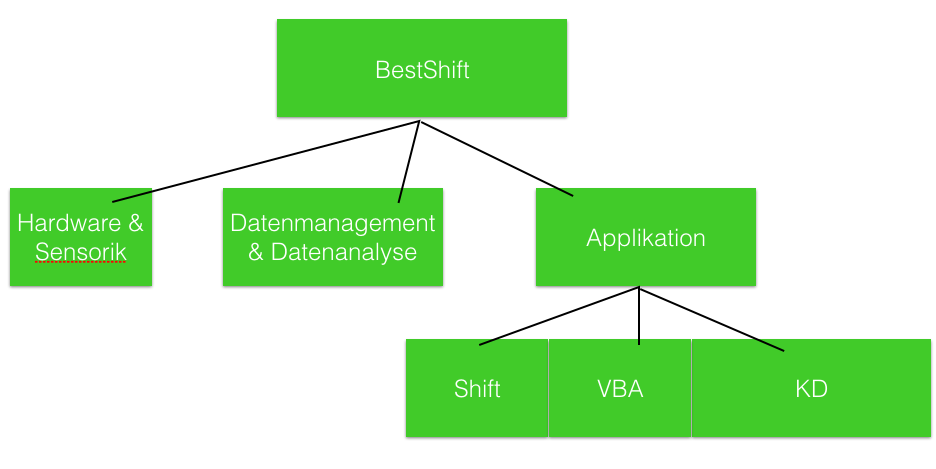
\includegraphics[height=0.28\textwidth]{images/Workflowdiagramm}
\end{center}
